\section{Modelos de datos}\label{sec:modelo}
Los modelos de datos son una representación estructurada de la información
almacenada que se utiliza para almacenar, recuperar y manipular los datos de
forma eficiente. En este caso, se definirán los modelos de datos que se
ingestarán en el sistema, así como las relaciones entre ellos y las
características de cada uno.

\emph{NOTA: debido a cuestiones de confidencialidad, no se mostrarán los modelos
de datos internos de Okticket.}

\subsection{Logs de balanceadores (AWS)}
\begin{figure}[H]
	\centering
	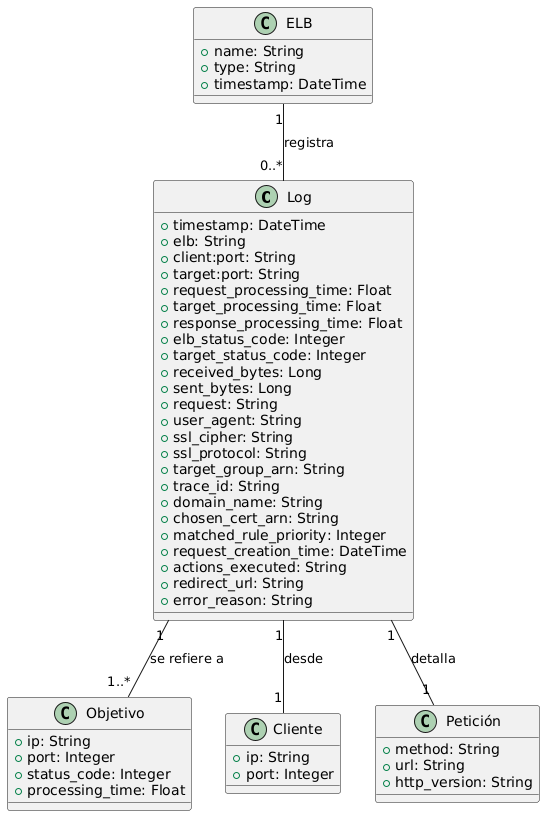
\includegraphics[width=0.65\textwidth]{uml/logs_elb.png}
	\caption{Modelo de datos de los logs de un balanceador de carga de AWS}
	\label{fig:logs_elb}
\end{figure}


\newpage{}
\subsection{Logs de bases de datos SQL}
\begin{figure}[H]
	\centering
	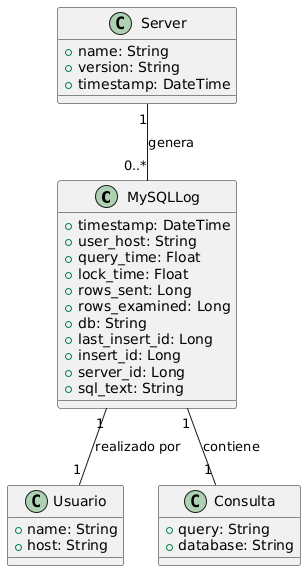
\includegraphics[width=0.4\textwidth]{uml/logs_sql.png}
	\caption{Modelo de datos de los logs de una base de datos SQL}
	\label{fig:logs_sql}
\end{figure}


\newpage{}
\subsection{Logs de bases de datos MongoDB}
\begin{figure}[H]
	\centering
	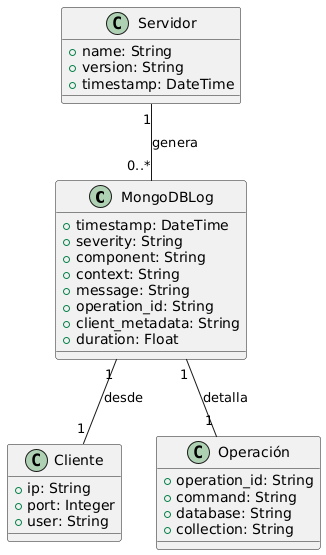
\includegraphics[width=0.4\textwidth]{uml/logs_mongo.png}
	\caption{Modelo de datos de los logs de una base de datos MongoDB}
	\label{fig:logs_mongo}
\end{figure}


\newpage{}
\subsection{Logs de Larvel (API)}
\begin{figure}[H]
	\centering
	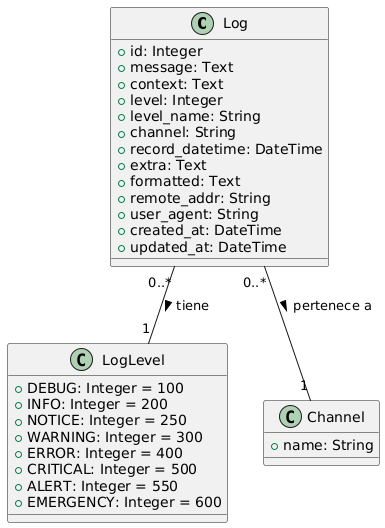
\includegraphics[width=0.5\textwidth]{uml/logs_laravel.png}
	\caption{Modelo de datos de los logs de una aplicación Laravel}
	\label{fig:logs_laravel}
\end{figure}
